\documentclass{article}

\usepackage{fancyhdr}
\usepackage{extramarks}
\usepackage{amsmath}
\usepackage{amsthm}
\usepackage{amsfonts}
\usepackage{tikz}
\usepackage[plain]{algorithm}
\usepackage{algpseudocode}
\usepackage{enumerate}
\usepackage{tikz}

\usetikzlibrary{automata,positioning}

%
% Basic Document Settings
%  

\topmargin=-0.45in
\evensidemargin=0in
\oddsidemargin=0in
\textwidth=6.5in
\textheight=9.0in
\headsep=0.25in

\linespread{1.1}

\pagestyle{fancy}
\lhead{\hmwkAuthorName}
\chead{\hmwkClass : \hmwkTitle}
\rhead{\firstxmark}
\lfoot{\lastxmark}
\cfoot{\thepage}

\renewcommand\headrulewidth{0.4pt}
\renewcommand\footrulewidth{0.4pt}

\setlength\parindent{0pt}

%
% Create Problem Sections
%

\newcommand{\enterProblemHeader}[1]{
    \nobreak\extramarks{}{Problem \arabic{#1} continued on next page\ldots}\nobreak{}
    \nobreak\extramarks{Problem \arabic{#1} (continued)}{Problem \arabic{#1} continued on next page\ldots}\nobreak{}
}

\newcommand{\exitProblemHeader}[1]{
    \nobreak\extramarks{Problem \arabic{#1} (continued)}{Problem \arabic{#1} continued on next page\ldots}\nobreak{}
    \stepcounter{#1}
    \nobreak\extramarks{Problem \arabic{#1}}{}\nobreak{}
}

\newcommand*\circled[1]{\tikz[baseline=(char.base)]{
		\node[shape=circle,draw,inner sep=2pt] (char) {#1};}}


\setcounter{secnumdepth}{0}
\newcounter{partCounter}
\newcounter{homeworkProblemCounter}
\setcounter{homeworkProblemCounter}{1}
\nobreak\extramarks{Problem \arabic{homeworkProblemCounter}}{}\nobreak{}

%
% Homework Problem Environment
%
% This environment takes an optional argument. When given, it will adjust the
% problem counter. This is useful for when the problems given for your
% assignment aren't sequential. See the last 3 problems of this template for an
% example.
%

\newenvironment{homeworkProblem}[1][-1]{
    \ifnum#1>0
        \setcounter{homeworkProblemCounter}{#1}
    \fi
    \section{Problem \arabic{homeworkProblemCounter}}
    \setcounter{partCounter}{1}
    \enterProblemHeader{homeworkProblemCounter}
}{
    \exitProblemHeader{homeworkProblemCounter}
}

%
% Homework Details
%   - Title
%   - Class
%   - Due date
%   - Name
%   - Student ID

\newcommand{\hmwkTitle}{Homework\ \#02}
\newcommand{\hmwkClass}{Probability \& Statistics for EECS}
\newcommand{\hmwkDueDate}{Feb 26, 2023}
\newcommand{\hmwkAuthorName}{Penghao Wang}
\newcommand{\hmwkAuthorID}{2021533138}


%
% Title Page
%

\title{
    \vspace{2in}
    \textmd{\textbf{\hmwkClass:\\  \hmwkTitle}}\\
    \normalsize\vspace{0.1in}\small{Due\ on\ \hmwkDueDate\ at 23:59}\\
	\vspace{4in}
}

\author{
	Name: \textbf{\hmwkAuthorName} \\
	Student ID: \hmwkAuthorID}
\date{}

\renewcommand{\part}[1]{\textbf{\large Part \Alph{partCounter}}\stepcounter{partCounter}\\}

%
% Various Helper Commands
%

% Useful for algorithms
\newcommand{\alg}[1]{\textsc{\bfseries \footnotesize #1}}
% For derivatives
\newcommand{\deriv}[1]{\frac{\mathrm{d}}{\mathrm{d}x} (#1)}
% For partial derivatives
\newcommand{\pderiv}[2]{\frac{\partial}{\partial #1} (#2)}
% Integral dx
\newcommand{\dx}{\mathrm{d}x}
% Alias for the Solution section header
\newcommand{\solution}{\textbf{\large Solution}}
% Probability commands: Expectation, Variance, Covariance, Bias
\newcommand{\E}{\mathrm{E}}
\newcommand{\Var}{\mathrm{Var}}
\newcommand{\Cov}{\mathrm{Cov}}
\newcommand{\Bias}{\mathrm{Bias}}

\begin{document}

\maketitle

\pagebreak

\begin{homeworkProblem}[1]
\begin{enumerate}
    \item As there the definiton of the bootstrap is a sequence formed from the $a_j$'s sampling with replacement, then as for $(a_1, ..., a_n)$, the number of possible bootstrap samples is $n*n*...*n = n^n$.
    \item As order does not matter, then we need to consider the choose times of each numbers, note that the sum of total choose times of all the numberes is $n$. Then this problem can be considered as partition of $n$ into $k$ parts and the number of ways to partition $n$ into $k$ parts is $\binom{n+k-1}{k-1}$. Here we consider that $k = n$, so the total number is $\binom{2n-1}{n-1}$. 
    \item 
    \begin{enumerate}
        \item Consider such 2 conditions: $b_1 = (a_1, a_2, ..., a_n)$, $b_2 = (a_1, a_1, ..., a_1)$. As order does not matter, then there are $n!$ cases of $b_1$, but as for $b_1$, there is only 1 cases. So we find the 2 samples and shows that not all unordered bootstrap samples are equally likely. 
        \item As defined below, we can find that the probability $p_1$ of $b_1$ is $\dfrac{n!}{n^n}$, and the probability $p_2$ of $b_2$ is $\dfrac{1}{n^n}$. Then we can calculate $p_1/p_2 = n!$. 
        \item As for the case $b_1$, there is only one case. But as for the case $b_2$, there is n cases as there is totally n numbers. Then the ratio is $\dfrac{\dfrac{n!}{n^n}}{\dfrac{n}{n^n}} = \dfrac{n!}{n}$, so the ratio is $(n-1)!$. 
    \end{enumerate}
\end{enumerate}
\end{homeworkProblem}

\newpage

\begin{homeworkProblem}[2]
    As for all the cases, there is totally $108^n$ cases. Then we define that event $A_i$ is that n boxes do not include 1 type coupons, event $C$ is that choose all 108 types of coupons. Then we then use the inclusion-exclusion formula, we have $P(C^c) = P(\cup_{i=1} ^{108} A_i) = \sum_iP(A_i) - \sum_{i<j}P(A_i \cap A_j) + ... + (-1)^{109}P(A_1 \cap ... \cap A_n) = \dfrac{\begin{pmatrix} 108 \\ 1 \end{pmatrix} 107^n }{108^n} - \dfrac{\begin{pmatrix} 108 \\ 2 \end{pmatrix} 106^n }{108^n} + ... + \dfrac{\begin{pmatrix} 108 \\ 107 \end{pmatrix} 1^n }{108^n} - \dfrac{0^n}{108^n} = \dfrac{\sum_{i=1}^{107}{\begin{pmatrix}108 \\ i \end{pmatrix}(-1)^{i+1}(108 - i) ^n}}{108^n}$. Then we have $P(C) = 1 - \dfrac{\sum_{i=1}^{107}{\begin{pmatrix}108 \\ i \end{pmatrix}(-1)^{i+1}(108 - i) ^n}}{108^n}$. As shown in the following figure, we can conclude that the when such probability is no less than 95\%, the minimum number of n is 823. \\
    \begin{figure}[htbp]
        \centering
        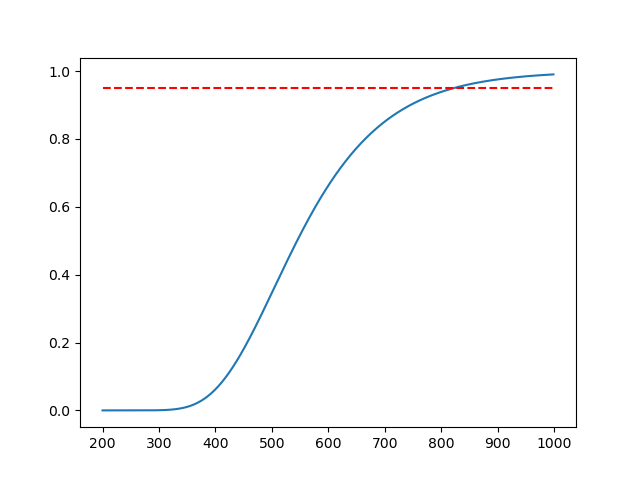
\includegraphics[width=1\textwidth]{Figure_1.png}
        \caption{The probability of choose all 108 types of coupons, n range from 200 to 1000}
        \label{fig:2}
    \end{figure}
\end{homeworkProblem}

\newpage

\begin{homeworkProblem}[3]
    Firstly choose four objects from the 100 garage kits, as there is 5 defectives, then the probability of accepted is choose the four kits from the 95 kits, that is $P = \dfrac{\begin{pmatrix} 95 \\ 4 \end{pmatrix}}{\begin{pmatrix} 100 \\ 4 \end{pmatrix}} = \dfrac{636709}{784245}$
\end{homeworkProblem}

\newpage

\begin{homeworkProblem}[4]
    Define event $A$ is first time draw a gold coin, define event $B$ is at the second draw, draw a gold coin, define $C_0$ as the event of take the box a, $C_1$ as the box b, $C_2$ as the box c. Then the probability $P(B|A) = \dfrac{P(B \cap A)}{P(A)} = \dfrac{P(B \cap A)}{P(A|C_0) + P(A|C_1) + P(A|C_2)} = \dfrac{\dfrac{1}{3}}{\dfrac{1}{3} + 0 + \dfrac{1}{3} * \dfrac{1}{2}} = \dfrac{2}{3}$
\end{homeworkProblem}

\newpage

\begin{homeworkProblem}[5]
    \begin{enumerate}
        \item As when Mirana play bold, Mirana won't draw, she wins with probability $p_w$, then loses with probability $(1-p_w)$, then there are 2 cases:
        \begin{enumerate}
            \item Win both in games 1 and 2, then the probability is $p_w * p_w = p_w^2$.
            \item Win a game and lose a game, then win in the third game, then the probability is $2 * p_w * (1-p_w) * p_w = 2p_w^2(1-p_w)$.
        \end{enumerate}
        Then the total probability is $p_w^2 + 2p_w^2(1-p_w) = p_w^2(3 - 2 p_w)$.
        \item As when Mirana play timid, Mirana won't win, she draws with probability $p_d$, then loses with probability $(1-p_d)$, then there is only 1 case:\\
        Draw both in games 1 and 2, then at games 3, Mirana play bold, and wins. The probability is $p_d * p_d * p_w = p_d^2p_w$. 
        \item As when Mirana play timid, Mirana won't win, she draws with probability $p_d$, then loses with probability $(1-p_d)$, and firstly Mirana plays bold then there are 3 case:
        \begin{enumerate}
            \item Win in game 1, draw in game 2. The probability is $p_w * p_d = p_wp_d$.
            \item Win in game 1. lose in game 2, then win in game 3. Then the probability is $p_w * (1 - p_d) * p_w = p_w^2 - p_w^2p_d$.
            \item Lose in game 1, win in game 2, then win in game 3. Then the probability is $(1 - p_w) * p_w * p_w = p_w^2 - p_w^3$. 
        \end{enumerate} 
        Add the three cases together, we will get that Mirana wins the match with probability $(p_wp_d) + (p_w^2 - p_w^2p_d) + (p_w^2 - p_w^3) = p_wp_d + 2p_w^2 - p_w^2p_d - p_w^3$.
        \item With the strategy in (c) above, we will get that, Mirana wins the match with probability $p_wp_d + 2p_w^2 - p_w^2p_d - p_w^3$. Then we analyse the probability:
        $p_wp_d + 2p_w^2 - p_w^2p_d - p_w^3 $.
        To make the probability big than 1/2, we can calculate the probability by give an example of $p_w$, $p_d$. Take $p_w = \dfrac{9}{20}$, $p_d = \dfrac{19}{20}$, we will get that the win probability is $\dfrac{549}{1000}$, where have a better than a 50-50 chance to win the match. 
        Intuitively, we can make partial derivative for $p_d$, then we will get that $p_w - p_w^2$, as $0 < p_w < \dfrac{1}{2}$, then we will get that the derivative bigger than 0, so the probability will grow bigger as $p_d$ grow bigger. As we have get a example that make the probability bigger than $\dfrac{1}{2}$, so there may have the chance. Also, as Mirana plays timid when she get ahead, and bold when she get behind, which increase the probablity of Mirana wins, when ahead, she play timid to decrease the probablity to fall behind, when behind, plays bold to increase the probablity to win in order to get ahead, so the probability will may bigger than $\dfrac{1}{2}$.
    \end{enumerate}
\end{homeworkProblem}
\end{document}
